Let \( \mathcal{R} = \mathcal{A} \cup \mathcal{B} \) be a set of DPO rewriting rules and let $\mathcal{T}=(T,\mathbb{E},\mathcal{S},w)$ be a finitary weighted type graph over a well-founded commutative semiring such that for every graph $G$ subject to rewriting, we have $\operatorname{Hom}(G,T)\neq \emptyset$. By \autoref{rem:wf:weight_of_object_geq_1}, for all objects \( G \) subject to rewriting, \(w_\mathcal{T}(G) \succeq_S 1_\mathcal{S} \).

The rewriting relation \( \Rightarrow_{\mathcal{A},\mathfrak{F}} \) is terminating relative to $\Rightarrow_{\mathcal{B},\mathfrak{F}}$ if (i) for all \(G \Rightarrow_{\mathcal{A},\mathfrak{F}} H\), \( w_\mathcal{T}(G) \succ_S w_\mathcal{T}(H)\), and (ii) for all \(G \Rightarrow_{\mathcal{B},\mathfrak{F}} H\), \( w_\mathcal{T}(G) \succeq_S w_\mathcal{T}(H) \). However, directly verifying all rewriting steps is infeasible due to the potentially infinite number of rewriting steps.

In this section, we recall the concepts of traceability of objects (Definition \ref{def:traceability}) and relative monicity of morphisms (\autoref{def:relative_monicity}), which are used to define the notion of weighable pushout squares (\autoref{def:weighable}). Using the notion of a weighable pushout square, we can bound the weight of the pushout object as explained below.

\noindent
\begin{minipage}{0.7\textwidth}\setlength{\parindent}{1em}
    Consider a DPO diagram (illustrated on the right) that defines a rewriting step \( G \Rightarrow_{\rho,\mathfrak{F}} H \). 
    If the left pushout square is weighable with $\mathcal{T}$ and the right pushout square is bounded above by $\mathcal{T}$ (concepts defined in \autoref{def:weighable}), then, by \cite[Lemma 4.13]{endrullis2024generalized_arxiv_v2}, we obtain:
\end{minipage}%
\hfill
\begin{minipage}{0.29\textwidth}
    \hfill
    \resizebox{\textwidth}{!}{
    \begin{tikzpicture}
        % [node distance=11mm]
        \node (I) at (0,0) {$K$};
        \node (L) at (-2,0) {$L$};
        \node (R) at (2,0) {$R$};
        \node (G) at (-2,-2) {$G$};
        \node (C) at (0,-2) {$C$};
        \node (H) at (2,-2) {$H$};
        \draw [->] (I) to  node [midway,below] {$l$} (L);
        \draw [->] (I) to  node [midway,below] {$r$} (R);
        \draw [->] (L) to node [midway,right] {$m$} (G);
        \draw [->] (I) to node [midway,right] {$u$} (C);
        \draw [->] (R) to node [midway,left] {$m'$} (H);
        \draw [->] (C) to node [midway,above] {$l'$} (G);
        \draw [->] (C) to node [midway,above] {$r'$} (H);
        \node [at=($(I)!.5!(G)$)] {\normalfont PO};
        \node [at=($(I)!.5!(H)$)] {\normalfont PO};
      \end{tikzpicture}
    }
\end{minipage}

% \begin{flalign*}
%     w_\mathcal{T}(G) 
%         & \overset{def}{=} \bigoplus_{t_G: G \rightarrow T} w_\mathcal{T}(t_G) 
%         \overset{def}{=} \bigoplus_{t_K: K \rightarrow T} \bigoplus_{\substack{t_G: G \rightarrow T\\ t_K = l \star m \star t_G}} w_\mathcal{T}(t_G) \\
%     w_\mathcal{T}(H) 
%         &\overset{def}{=} \bigoplus_{t_H: H \rightarrow T} w_\mathcal{T}(t_H) 
%          \overset{def}{=} \bigoplus_{t_K: K \rightarrow T} \bigoplus_{\substack{t_H: H \rightarrow T\\ t_K = r \star m' \star t_H}} w_\mathcal{T}(t_H)
% \end{flalign*}

% If the left pushout square is weighable with $\mathcal{T}$ and the right pushout square is bounded above by $\mathcal{T}$ (concepts defined in \autoref{def:weighable}), then, by \cite[Lemma 5.10]{endrullis2024generalized_lmcs}, we derive the following assertions:
% \begin{flalign*}
%     w_\mathcal{T}(G) 
%         & = \bigoplus_{t_K: K \rightarrow T} \bigoplus_{\substack{t_G: G \rightarrow T\\ t_K = l \star m \star t_G}} w_\mathcal{T}(m \star t_G) \odot (l' \star t_G - u) \\
%     w_\mathcal{T}(H) 
%         &  \preceq \bigoplus_{t_K: K \rightarrow T} \bigoplus_{\substack{t_H: H \rightarrow T\\ t_K = r \star m' \star t_H}} w_\mathcal{T}(m' \star t_H) \odot (r' \star t_H - u)
% \end{flalign*}
% By \cite[Theorem 5.12]{endrullis2024generalized_lmcs}, it follows:
% \begin{flalign*}
%     w_\mathcal{T}(G) 
%         & = \bigoplus_{t_K: K \rightarrow T} 
%         \bigoplus_{\substack{t_C: C \rightarrow T\\ t_K = u \star t_C}}
%         \bigoplus_{\substack{t_L: L \rightarrow T\\ t_K = l \star t_L}}
%             w_\mathcal{T}(t_L) \odot w_\mathcal{T}(t_C - u) \\
%     w_\mathcal{T}(H) 
%         &  \preceq \bigoplus_{t_K: K \rightarrow T} 
%         \bigoplus_{\substack{t_C: C \rightarrow T\\ t_K = u \star t_C}}
%         \bigoplus_{\substack{t_R: R \rightarrow T\\ t_K = r \star t_R}}
%             w_\mathcal{T}(t_R) \odot w_\mathcal{T}(t_C - u) \\
% \end{flalign*}
% By \cite[Theorem 5.13]{endrullis2024generalized_lmcs}, we have the following assertions: 
\begin{flalign*}
    w_\mathcal{T}(G) 
        & = \bigoplus_{t_K: K \rightarrow T} 
        \left ( \bigoplus_{\substack{t_C: C \rightarrow T\\ t_K = u \star t_C}}
          w_\mathcal{T}(t_C - u) \right ) 
          \odot
        \left (\bigoplus_{\substack{t_L: L \rightarrow T\\ t_K = l \star t_L}}
        w_\mathcal{T}(t_L) \right )
         \\
    w_\mathcal{T}(H) 
        &  \preceq \bigoplus_{t_K: K \rightarrow T} 
        \left ( \bigoplus_{\substack{t_C: C \rightarrow T\\ t_K = u \star t_C}}
         w_\mathcal{T}(t_C - u) \right ) 
         \odot 
         \left ( \bigoplus_{\substack{t_R: R \rightarrow T\\ t_K = r \star t_R}}
            w_\mathcal{T}(t_R) \right ) \\
\end{flalign*}
According to these results, a termination criterion will be established in~\textsection~\ref{wf:sec:termination} by comparing the weights 
$\bigoplus_{\substack{t_L: L \rightarrow T\\ t_K = l \star t_L}}
        w_\mathcal{T}(t_L)$ and 
$\bigoplus_{\substack{t_R: R \rightarrow T\\ t_K = r \star t_R}} 
        w_\mathcal{T}(t_R)$ for every $t_K: K \rightarrow T$.

\begin{definition}[Traceability~\cite{endrullis2024generalized_arxiv_v2}]
    \label{def:traceability}
    \ \newline
\noindent 
\begin{minipage}{0.5\textwidth}
An object $X \in \mathcal{C}$ is called \emph{traceable} along a class of pushout squares $\Delta$ if for every diagram $\delta \in \Delta$ (shown on the right), the following hold
\end{minipage}
\hfill
\begin{minipage}{0.5\textwidth}
    \hfill
    \resizebox{0.9\textwidth}{!}{
    \begin{tikzpicture}
      \node (A) at (0,0) {$A$};
      \node (B) at (2,0) {$B$}; 
      \node  (C) at (0,-2) {$C$}; 
      \node  (D) at (2,-2) {$D$}; 
      \node  (X) at (4,-2) {$X$};
      \begin{scope}[nodes=rectangle]          
      \draw [->] (A) to node [above,label,pos=0.5] {$\alpha$} (B);
      \draw [->] (A) to node [left,label,pos=0.5] {$\beta$} (C);
      \draw [->] (B) to node [right,label,pos=0.45] {$\beta'$} (D); 
      \draw [->] (C) to node [below,label,pos=0.45] {$\alpha'$} (D);
      \draw [->] (X) to node [below,label,pos=0.4] {$h$} (D);
      \end{scope}
      \node at ($(A)!.5!(D)$) {$\delta$};
    \end{tikzpicture}
    }
\end{minipage}
    \begin{enumerate}[label=(\alph*)]
        \item\label{traceable:a} there exists a morphism $f : X \to B$ such that $h = f \star \beta'$, or
        \item\label{traceable:b} there exists a morphism $g : X \to C$ such that $h = g \star \alpha'$.
    \end{enumerate}
    If additionally, 
    whenever \ref{traceable:a} and \ref {traceable:b} hold,
    \begin{enumerate}[label=(\alph*),resume]
        \item 
        there exists a morphism $k : X \to A$ such that $h = k \star \alpha \star \beta' $,
    \end{enumerate}
    then we say that $X$ is \emph{$\beta$-strongly traceable} along $\Delta$.
\end{definition}
Consider the category \textbf{Graph}. Intuitively, a graph $X$ is $\beta$-strongly traceable along a pushout square as illustrated above, if whenever $X$ occurs in $D$, it occurs either in $B$ or in $C$, and if it occurs in both, then it occurs in $A$ as well.

\begin{remark}[~\cite{endrullis2024generalized_arxiv_v2}]
    \label{remark:traceability_graph}
    In \textbf{Graph}, the objects \tikz[baseline=-0.5ex]{
        \node[draw,circle] (x) at (0,0) {};
    } and
    %  \tikz[baseline=-0.5ex]{
    %     \node (x) at (0,0) {$\bullet$};
    %     \node (y) at (1,0) {$\bullet$};
    %     \draw[->] (x) -- (y) node[midway, above] {$x$};
    % } 
    \raisebox{2pt}{
            \scalebox{0.7}{\tikz[baseline=-0.5ex]{
            \node[draw,circle] (x) at (0,0) {};
            \node[draw,circle] (y) at (1,0) {};
            \draw[->] (x)--(y) node[midway, above] {$x$};
        }}}
    (for edge labels $x$) are the only (non-initial) objects that are (strongly) traceable along all pushout squares. 
    Other objects, such as loops~\tikz[baseline=-0.5ex]{
        \node[draw,circle] (x) at (0,0) {};
        \draw[->] (x) edge[loop right]  node[midway, right] {$x$}  (x)
    }, are strongly traceable if all morphisms in the square are monomorphisms.
\end{remark}

\begin{example}
    Consider the DPO diagram shown in~\autoref{fig:nwf:two_pushout_squares}.
    \begin{figure}
        \centering 
      \resizebox{0.7\textwidth}{!}{
      \begin{tikzpicture}
          \graphbox{\( L \)}{0mm}{-3mm}{34mm}{12mm}{2mm}{2mm}{
              \coordinate (o) at (0mm,-8mm); 
              \node[draw,circle] (l1) at ($(o)+(-10mm,0mm)$) {1};
              \node[draw,circle] (l2) at ($(l1)+(2,0)$) {2};
              \node[draw,circle] (l3) at ($(l1) + (1,0)$) {3};
              \draw[] (l1) -- (l3) node[midway,above] {a};
              \draw[] (l3) -- (l2) node[midway,above] {a};
          } 
          \graphbox{\( K \)}{40mm}{-3mm}{34mm}{12mm}{2mm}{2mm}{
              \coordinate (o) at (0mm,-8mm); 
              \node[draw,circle] (l1) at ($(o)+(-10mm,0mm)$) {1};
              \node[draw,circle] (l2) at ($(l1)+(2,0)$) {2};
          }  
          \graphbox{\( R \)}{80mm}{-3mm}{45mm}{12mm}{2mm}{2mm}{
              \coordinate (o) at (-5mm,-8mm); 
              \node[draw,circle] (l1) at ($(o)+(-10mm,0mm)$) {1};
              \node[draw,circle] (l2) at ($(l1)+(3,0)$) {2};
              \node[draw,circle] (l3) at ($(l1) + (1,0)$) {4};
              \node[draw,circle] (l4) at ($(l1) + (2,0)$) {5};
              \draw[ ] (l1) -- (l3) node[midway,above] {a};
              \draw[ ] (l3) -- (l4) node[midway,above] {b};
              \draw[ ] (l4) -- (l2) node[midway,above] {a};
          }    
          \graphbox{\( G \)}{0mm}{-22mm}{34mm}{22mm}{2mm}{-3mm}{
              \coordinate (o) at (0mm,-3mm); 
              \node[draw,circle] (l1) at ($(o)+(-10mm,0mm)$) {1};
              \node[draw,circle] (l2) at ($(l1)+(2,0)$) {2};
              \node[draw,circle] (l3) at ($(l1) + (1,0)$) {3};
              \node[draw,circle] (l4) at ($(l2) + (0,-1)$) {6};
              \draw[] (l1) -- (l3) node[midway,above] {a};
              \draw[] (l3) -- (l2) node[midway,above] {a};
              \draw[ ] (l2) -- (l4) node[midway,right] {a};
              \node[draw,circle] (l6) at ($(l1) + (0,-1)$) {7};
              \draw[] (l1) -- (l6) node[midway,left] {a};
          }    
          \graphbox{\( C  \)}{40mm}{-22mm}{34mm}{22mm}{2mm}{-3mm}{
              \coordinate (o) at (0mm,-3mm); 
              \node[draw,circle] (l1) at ($(o)+(-10mm,0mm)$) {1};
              \node[draw,circle] (l2) at ($(l1)+(2,0)$) {2};
              \node[draw,circle] (l4) at ($(l2) + (0,-1)$) {6};
              \draw[ ] (l2) -- (l4) node[midway,right] {a};
              \node[ draw,circle] (l6) at ($(l1) + (0,-1)$) {7};
              \draw[ ] (l1) -- (l6) node[midway,left] {a};
          }    
          \graphbox{\( H \)}{80mm}{-22mm}{45mm}{22mm}{2mm}{-3mm}{
              \coordinate (o) at (-5mm,-3mm); 
              \node[draw,circle] (l1) at ($(o)+(-10mm,0mm)$) {1};
              \node[draw,circle] (l2) at ($(l1)+(3,0)$) {2};
              \node[draw,circle] (l3) at ($(l1) + (1,0)$) {4};
              \node[draw,circle] (l4) at ($(l1) + (2,0)$) {5};
              \node[ draw,circle] (l5) at ($(l2) + (0,-1)$) {6};
              \node[ draw,circle] (l6) at ($(l1) + (0,-1)$) {7};
              \draw[ ] (l1) -- (l6) node[midway,left] {a};
              \draw[] (l1) -- (l3) node[midway,above] {a};
              \draw[] (l3) -- (l4) node[midway,above] {b};
              \draw[ ] (l4) -- (l2) node[midway,above] {a};
              \draw[ ] (l2) -- (l5) node[midway,right] {a};
          }    
          \node () at (37mm,-8mm) {\( \leftarrowtail \)}; % K -> L
          \node () at (77mm,-8mm) {\( \rightarrowtail \)}; % K -> R
          \node () at (15mm,-18mm) {\( m\ \downarrowtail \)};
          \node () at (37mm,-33mm) {\( \leftarrowtail \)};
          \node () at (58mm,-18mm) {\( u\downarrowtail \)};
          \node () at (102mm,-18mm) {\( \downarrowtail \)};
          \node () at (77mm,-33mm) {\( \rightarrowtail \)}; % C -> H
      \end{tikzpicture}
      }
      \caption{}
      \label{fig:nwf:two_pushout_squares}
  \end{figure}
   The graph 
   \tikz[baseline=-0.5ex]{
        \node[draw,circle] (x) at (0,0) {};
        \node[draw,circle] (y) at (1,0) {};
        \node[draw,circle] (z) at (2,0) {};
        \draw[->] (x) -- (y) node[midway, above] {$a$};
        \draw[<-] (z) -- (y) node[midway, above] {$a$};
    } is not traceable in both pushout squares. The graph \tikz[baseline=-0.5ex]{
        \node[draw,circle] (x) at (0,0) {};
        \node[draw,circle] (y) at (1,0) {};
        \draw[->] (x) -- (y) node[midway, above] {$a$};
    } is traceable (and $u$-strongly traceable) along both pushout squares.
\end{example}

\begin{example} 
    Consider the rewriting step shown in~\autoref{fig:nwf:rewriting_step_traceability}.
    The graph 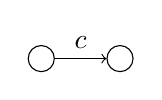
\begin{tikzpicture}
        \node[draw, circle] (x) at (0,0) {};
        \node[draw, circle] (y) at (1,0) {};
        \draw[->]  (x) -- (y) node [midway,above] {$c$};
    \end{tikzpicture} 
    is traceable along both pushout squares. 
     It is $u$-strongly traceable along the left pushout square, but not $u$-strongly traceable along the right pushout square. 
    The graph 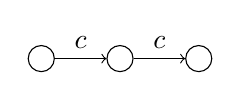
\begin{tikzpicture}
        \node[draw, circle] (x) at (0,0) {};
        \node[draw, circle] (y) at (1,0) {};
        \node[draw, circle] (z) at (2,0) {};
        \draw[->]  (x) -- (y) node [midway,above] {$c$};
        \draw[->]  (y) -- (z) node [midway,above] {$c$};
    \end{tikzpicture} is not traceable along both pushout squares.
%     because    
%     \begin{tikzpicture}
%        \node[draw, circle] (x) at (0,0) {z};
%        \node[draw, circle] (y) at (1,0) {x};
%        \node[draw, circle] (z) at (2,0) {y};
%        \draw[->]  (x) -- (y) node [midway,above] {$c$};
%        \draw[->]  (y) -- (z) node [midway,above] {$c$};
%    \end{tikzpicture} is in the pushout object $G$ but in neither $L$ nor $C$.
   \begin{figure}
    \centering
    \resizebox{0.7\textwidth}{!}{
    \begin{tikzpicture}
        \graphbox{$L$}{0mm}{0mm}{35mm}{35mm}{2mm}{-7mm}{
        \node[draw,circle] (1) at (0,0) {x};
        \node[draw,circle] (2) at (1,-2) {y};
        \node[draw,circle] (3) at (-1,-2) {z};
        \draw[->] (1) edge node[midway,right]  {c}  node[midway,left]{} (2);
        \draw[->] (2) edge node[midway,above]  {c}  node[midway,below]{}  (3);
        }
        \graphbox{$K$}{45mm}{0mm}{35mm}{35mm}{2mm}{-7mm}{
        % I
            % \def\x{5};
            % \def\y{0};
            \node[draw,circle] (1) at (0,0) {x};
            \node[draw,circle] (2) at (1,-2) {y};
            \node[draw,circle] (3) at (-1,-2) {z};
            \draw[->] (2) edge node[midway,above]  {c}  node[midway,below]{}  (3);
        }
        \node () at (40mm,-15mm)  {$\overset{l}{\leftarrowtail}$};

        % \node () at (2.5,-2.5) {PO};
        \graphbox{$R$}{90mm}{0mm}{35mm}{35mm}{2mm}{-7mm}{
        % R
            % \def\x{10};
            % \def\y{-1.1};
            \node[draw,circle] (1) at (0,-1) {x y z};
            \draw[->] (1) edge[loop below]  node[midway, above] {$c$}  (1);
        }
        \node () at (85mm,-15mm)  {$\overset{r}{\rightarrow}$};

        \graphbox{$G$}{0mm}{-45mm}{35mm}{35mm}{2mm}{-7mm}{
        % \node () at (7.5,-2.5) {PO};
        % G
            % \def\x{0};
            % \def\y{-5};
            \node[draw,circle] (1) at (0,0) {x};
            \node[draw,circle] (2) at (1,-2) {y};
            \node[draw,circle] (3) at (-1,-2) {z};
            \draw[->] (1) edge node[midway,right]  {c}  node[midway,left]{} (2);
            \draw[->] (2) edge node[midway,above]  {c}  node[midway,below]{}  (3);
            \draw[->] (3) edge node[midway,above]  {c}  node[midway,below]{}  (1);
        }
        % C
        \graphbox{$C$}{45mm}{-45mm}{35mm}{35mm}{2mm}{-7mm}
        {    
            \node[draw,circle] (1) at (0,0) {x};
            \node[draw,circle] (2) at (1,-2) {y};
            \node[draw,circle] (3) at (-1,-2) {z};
            % \draw[->] (1) edge node[midway,right]  {c}  node[midway,left]{} (2);
            \draw[->] (3) edge node[midway,above]  {c}  node[midway,below]{} (1);
            \draw[->] (2) edge node[midway,above]  {c}  node[midway,below]{} (3);
            }
        \node () at (40mm,-55mm)  {$\overset{l}{\leftarrowtail}$};
        % H
        \graphbox{$H$}{90mm}{-45mm}{35mm}{35mm}{2mm}{-7mm}{
        % R
            % \def\x{10};
            % \def\y{-1.1};
            \node[draw,circle] (1) at (0,-1) {x y z};
            \draw[->] (1) edge[loop below]  node[midway, below] {} node[midway, above] {$c$} (1);
            \draw[->] (1) edge[loop above]  node[midway, below] {} node[midway, above] {$c$} (1);
        }

        \node () at (85mm,-55mm)  {$\overset{r}{\rightarrow}$};
        \node () at (17mm,-40mm) {$m\downarrowtail$};
        \node () at (62mm,-40mm) {$u\downarrowtail$};
        \node () at (107mm,-40mm) {$\downarrow m'$};
    \end{tikzpicture}
    }
    \caption{}
    \label{fig:nwf:rewriting_step_traceability}
   \end{figure}
\end{example} 
The following concepts are restricted versions of the concept of monicity.
\begin{definition}[Relative Monicity~\cite{endrullis2024generalized_arxiv_v2}]
    \label{def:relative_monicity}
    Let $A,B,C$ and $X$ be objects, $\Gamma$ a set of objects, $S$ a set of morphisms to $A$ and $u:C\to A$ a morphism. A morphism $f : A \to B$ is called 
    \begin{enumerate}[label=(\roman*)] 
        \item 
            \emph{monic for $S$} 
            if $g \star f = h \star f$ implies $g = h$ for all $g, h \in S$;
        \item 
            \emph{$X$-monic} if $f$ is monic for $\operatorname{Hom}(X, A)$.
        \item \emph{$X$-monic outside of $u$}, if $f$ is monic for \( \operatorname{Hom}(X,A) \setminus \left ( \operatorname{Hom}(X,C) \star u \right ) \).
        \item  \emph{$\Gamma$-monic} if $f$ is $X$-monic for every $X \in \Gamma$.
    \end{enumerate}
\end{definition} 
\begin{example}[Edge-Monicity \cite{endrullis2024generalized_arxiv_v2}]
    In $\mathbf{Graph}$, let 
    $\Gamma = \left\{ \vcenter{\hbox{
    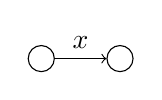
\begin{tikzpicture}[baseline=-0.5ex]
    \node[draw,circle] (A) at (0,0) {};
    \node[draw,circle] (B) at (1,0) {};
    \draw[->] (A) -- (B) node[midway, above] {$x$};
    \end{tikzpicture}
    }} \mid x \text{ is an edge label} \right\}$.
    A morphism $f : G \to H$ that does not identify edges (but may identify nodes) is not necessarily monic, but it is $\Gamma$-monic. 
\end{example}
\begin{definition}[Weighable Pushout Square~\text{\cite[\textdef~4.9]{endrullis2024generalized_arxiv_v2}}]
    \label{def:weighable}
    \ \newline
    \noindent
    \begin{minipage}{0.7\textwidth}
        Let  $\mathcal{T} = (T,\mathbb{E}, S, w)$ be a finitary weighted type graph.
        Consider the pushout square $\delta$ shown on the right. We say that $\delta$ is
         \begin{enumerate}[label=(\alph*)]
        \item \emph{weighable} with $\mathcal{T}$ if the following hold:
            \begin{enumerate}[label=(\roman*)]
                \item $dom(\mathbb{E})$ is strongly traceable along $\delta$,
                \item $\beta'$ is $dom(\mathbb{E})$-monic,
                \item $\alpha'$ is $dom(\mathbb{E})$-monic outside of $\beta$.
            \end{enumerate}
        \item \emph{bounded-above} by $\mathcal{T}$ if $dom(\mathbb{E})$ is traceable along $\delta$.
    \end{enumerate}
    \end{minipage}
    \begin{minipage}{0.3\textwidth}
        \begin{center}
            \begin{tikzpicture}[node distance=12mm]
                \node (A) {$A$};
                \node (B) [right of=A] {$B$};
                \node (C) [below of=A] {$C$};
                \node (D) [right of=C] {$D$};
                \draw [->] (A) to node [above, label] {$\alpha$} (B);
                \draw [->] (A) to node [left, label] {$\beta$} (C);
                \draw [->] (B) to node [right, label] {$\beta'$} (D);
                \draw [->] (C) to node [below, label] {$\alpha'$} (D);
                \node [at=($(A)!.5!(D)$)] {$\delta$};
            \end{tikzpicture}
        \end{center}
    \end{minipage}
   
\end{definition}

